\begin{figure}[!htb]
    \centering
    \resizebox{0.48\textwidth}{!}{%
        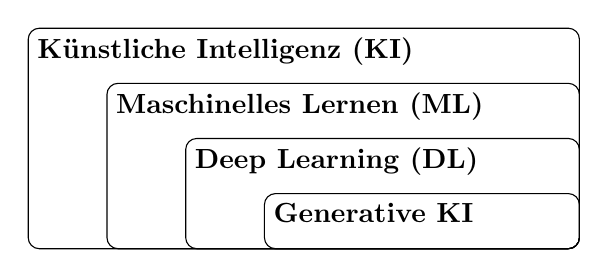
\begin{tikzpicture}
            \node[rectangle, draw, rounded corners, minimum height=2.8cm, minimum width=7cm] (ai) {};

            \node[rectangle, draw, rounded corners, minimum height=2.1cm, minimum width=6cm, anchor=south east] (ml) at (ai.south east) {};

            \node[rectangle, draw, rounded corners, minimum height=1.4cm, minimum width=5cm, anchor=south east] (dl) at (ml.south east) {};

            \node[rectangle, draw, rounded corners, minimum height=0.7cm, minimum width=4cm, anchor=south east] (genai) at (dl.south east) {};

            \node[anchor=north west] at (ai.north west) {
                \textbf{Künstliche Intelligenz (KI)}
            };

            \node[anchor=north west] at (ml.north west) {
                \textbf{Maschinelles Lernen (ML)}
            };

            \node[anchor=north west] at (dl.north west) {
                \textbf{Deep Learning (DL)}
            };

            \node[anchor=north west] at (genai.north west) {
                \textbf{Generative KI}
            };
        \end{tikzpicture}
    }
    \caption{Begriffe im Rahmen von künstlicher Intelligenz.}
    \label{sec1:intro:fig:ai-terms}
\end{figure}